%!TEX root = ../dokumentation.tex

\chapter{Umsetzung}

Nach dem der Schritt der Planung und der Analyse abgeschlossen ist, kann es nun
weiter zur tatsächlichen Entwicklung gehen. Dazu müssen zunächst die einzelnen
Entwicklungsumgebungen vorbereitet werden, anschließend die ersten Konzepte für
die Umsetzung aufgestellt werden, bis es abschließend zur tatsächlichen
Realisierung kommt. 

%title wird unter dem Bsp. abgedruckt
%caption wird im Verzeichnis abgedruckt
%label wird zum referenzieren benutzt, muss einzigartig sein.

\section{Voraussetzungen}
Für die Nutzung des Audioplayer auf dem Raspberry Pi bzw. für die weitere
Entwicklung, müssen vorerst einige Anpassungen und Installationen getätigt
werden. Diese Schritte sind notwendig damit der Audioplayer wie vorgesehen
funktioniert und keine unvorhergesehen Zustände entstehen.

\subsection{Pakete installieren und Raspberry Pi updaten}
Standardmäßig besitzt der Raspberry Pi das Betriebssystem \textit{Raspbian}.
Dieses gilt es zuerst auf die neuste Version zu aktualisieren. Zusätzlich
werden alle installierten Pakete des System auf die neuste Version zu
aktualisieren. Dieses Vorhaben wird mit den folgenden Befehlen durchgeführt:
\begin{lstlisting}[caption={Aktualisieren des Raspberry Pi}]
sudo apt-get update 
sudo apt-get upgrade 
sudo apt-get install rpi-update 
sudo rpi-update
\end{lstlisting}
Die ersten drei Befehle werden mit \ac{APT} ausgeführt. \ac{APT} ist ein
Paketverwaltungssystem welches für den Bereich der Debian Betriebssysteme
entwickelt wurde. Das Tool verwaltet Debian Pakete und somit auch die
installierten Applikationen auf dem Raspberry Pi
\autocite{apt-debian-wiki_2019}. Zusätzlich wird für alle durchzuführende
Befehle der \verb|sudo| Befehl benutzt. \ac{Sudo} wird meistens dafür benutzt
bestimmte Befehle mit Root-Rechten also mit Administratorrechten auszuführen.
Der Vorteil liegt darin, dass der Nutzer eben nicht ein Administrator sein
muss, um kurzfristig einen Befehl als Administrator auszuführen
\autocite{moeller_2013}. Mit dem Befehl \verb|sudo apt-get update| werden alle
Paketquellen neu eingelesen - also ein großes Lexikon wo man jedes Paket mit
der neusten zur Verfügung stehenden Version finden kann. Mit dem Befehl
\verb|sudo apt-get upgrade| werden alle bereits installierten Paket auf die in
den Paketquellen vorhandene neuste Version aktualisiert. Dabei werden keine
neuen Pakete installiert oder alte nicht mehr benötigte Abhängigkeiten
entfernt. \autocite{apt-get-wiki_2019} Mit dem Befehl \verb|apt-get install rpi-update| 
wird das Paket \verb|rpi-update| mit allen seinen Abhängigkeiten
heruntergeladen und installiert. Das Paket ist ein automatisiertes Skript zum
updaten des Raspberry Pi's Betriebssystem auf die neuste Version. Als letzten
Schritt wird nun das Paket \verb|rpi-update| ausgeführt und der Raspberry Pi
lädt automatisch das neuste passende Betriebssystem herunter und installiert
es. Dabei gehen keine Daten verloren. \\ Nachdem der Raspberry Pi sich
erfolgreich aktualisiert hat, müssen nun noch die jedenfalls benötigten Pakete
installiert werden. Dies wird mit den folgenden Befehlen gemacht.
\begin{lstlisting}[caption={Installation benötigter Pakete}]
sudo apt-get install portaudio19-dev
sudo apt-get install libmpg123-dev
sudo apt-get install mp3info 
\end{lstlisting}

\subsection{Nötige Schritte für Entwicklungszwecke}
Im folgenden wird auf die einzelnen Schritte eingegangen, die nötig sind um an
dem erstellten Programm weiter zu entwickeln. Dazu müssen die im Anschluss
stehenden Befehle auf dem Raspberry Pi ausgeführt werden.

\subsubsection{Installieren von Go}
Nun wird auf die Installation von Go eingegangen.

\begin{enumerate}
\item \textbf{Herunterladen von Go} \\
Als ersten Schritt gilt es die Programmiersprache Go auf den Raspberry Pi
herunterzuladen. Dazu stellt der Hersteller offizielle Pakete für die
unterschiedlichen Betriebssysteme und Architekturen zum Download bereit. Diese
können über die \href{https://golang.org/dl/}{Download-Webseite}
heruntergeladen werden. In diesem Fall wird für den Raspberry Pi das Paket für
das Betriebssystem \textit{Linux} mit der Architektur \textit{ARMv6} benötigt.
Nachdem das passende Paket auf der Webseite gefunden wurde, muss der
Direkt-Link zu dem Download in den Zwischenspeicher kopiert werden und
anschließend der folgende Befehl auf dem Raspberry Pi ausgeführt werden.
\begin{lstlisting}
Befehl: wget [LINK]
\end{lstlisting}

\item \textbf{Entpacken des Archivs} \\
Nachdem das offizielle Archiv für die Programmiersprache Go heruntergeladen
wurde, muss dieses nun nach den Pfad \verb|/user/local| entpackt werden. Für
das entpacken des Archivs wird das standardmäßige Archivierungsprogramm für
Linux \textit{\ac{Tar}} verwendet. Der große Vorteil eines tar-Archivs ist,
dass die Benutzerrechte einer Datei mit gesichert werden und diese beim
Entpacken auch wiederhergestellt werden \autocite{tar-wiki_2019}. Das entpacken
des Archivs wird durch den folgenden Befehl realisiert. Der Dateiname
entspricht hier der zuvor heruntergeladenen Datei.
\begin{lstlisting}
tar -C /usr/local -xzf [Filename]
\end{lstlisting}

\item \textbf{Setzen des Export-Pfad} \\
Damit das Betriebssystem Go auch System weit kennt, muss der Pfad zu der
ausführbaren Datei von Go in die PATH-Variable eingetragen werden. Die
\textit{PATH-Variable} ist eine Umgebungsvariable, die aus einer
Komma-separierten Liste von Ordnern besteht, die die Shell beim der Eingabe
eines Kommandos durchsucht \autocite{quigley_2000}. Dies bewirkt, dass von
jedem Standpunkt im System auf Go bzw. den Go Compiler zugegriffen werden kann.
\begin{lstlisting}
export PATH=\$PATH:/usr/local/go/bin
\end{lstlisting}

\item \textbf{Überprüfen der Go Installation auf Korrektheit} \\
Um nun zu Überprüfen, ob Go richtig installiert wurde und die Path-Variable
korrekt gesetzt wurde, wird nun durch den einfachen Befehl \verb|go version|
eine Abfrage an den Go Compiler zu seiner aktuellen Version erstellt. Wird
dabei eine gewisse Version angezeigt, ist Go richtig installiert und im System
integriert.
\begin{lstlisting}
go version -> "go version go x.x.x"
\end{lstlisting}

\item \textbf{Go-Ordnerstruktur anlegen} \\
Go empfiehlt es eine Gewisse Ordnerstruktur für die Go Projekte anzulegen.
Diese mit den folgenden Befehlen angelegt und besteht aus:
\begin{itemize}
\item \textbf{bin} - enthält alle Go-Executable's, die mit dem Befehl \verb|go install| installiert wurden.
\item \textbf{pkg} - enthält alle kompilierten Pakete, die in Projekte importiert werden können. 
\item \textbf{src} - enthält alle Quelldateien, entweder die eigenen oder aus externen Repositories heruntergeladene Quellen.
\end{itemize}
In der folgenden Übersicht wird die Ordnerstruktur nochmals visuell
dargestellt. Der Ordner \textit{pi} stellt hier den Nutzernamen da, der sich
bei jedem System natürlich unterscheiden kann. \\
\begin{minipage}[t]{\textwidth}
\dirtree{%
.1 /. 
.2 home. 
.3 pi. 
.4 go. 
.5 src. 
.5 pkg. 
.5 bin. 
}
Die Befehle zur Erstellung der Ordnerstruktur sehen wie folgt aus. \\
Ausgehend von \verb|$Home|:
\begin{lstlisting}[caption={Erstellung der Go Ordnerstruktur}]
mkdir go
cd go
mkdir src
mkdir pkg
mkdir bin
\end{lstlisting}
\end{minipage}


\end{enumerate}

\subsubsection{Klonen des Git Repository}
Der nächste Schritt ist das Git Repository auf den lokalen PC zu klonen. Go
schreibt dafür einen Standard vor, wie die Ordnerstruktur dazu bestenfalls
aufgebaut werden sollte. Im folgenden werden nun die Befehle zur Erstellung
Ordnerstruktur dargestellt. Diese Befehle Starten von \verb|/home/pi/go/src/|:
\begin{lstlisting}[caption={Klonen des Git Repository}]
mkdir github.com 
cd github.com
mkdir alexanderklapdor
cd alexanderklapdor
git clone https://github.com/alexanderklapdor/RaspberryPi_Go_Audioplayer.git
\end{lstlisting}

\subsubsection{Installieren der Go Abhängigkeiten}
Bei der Entwicklung des Audioplayers wurden weitere Go-Projekte verwendet,
welche nun für die Entwicklung auf den lokalen Rechner heruntergeladen werden
müssen. Um nicht alle Abhängigkeiten einzeln zu installieren, kann Go sich alle
benötigten Projekte alleine herunterladen. Dies wird durch den folgenden Befehl
gemacht.
Starting from \verb|../RaspberryPi_Go_Audioplayer/| :
\begin{lstlisting}
go get ./... 
\end{lstlisting}

\subsubsection{Modifizieren der ALSA Bibliothek Dateien}
Die Konfigurationdatei der ALSA Bibliothek muss editiert werden damit die
Fehlermeldungen, welche durch die nicht vorhandenen Anschlüsse am Raspberry Pi
hervorgerufen werden, nicht immer mit ausgegeben werden. \\
Zugriff auf die Datei wird mit dem Befehl \verb|sudo nano /usr/share/alsa/alsa.conf|  \\
Folgende Einträge müssen aus dieser Datei entfernt werden:
\begin{lstlisting}[caption={Liste der zu löschenden Einträge}]
pcm.rear cards.pcm.rear 
pcm.center_lfe cards.pcm.center_lfe 
pcm.side cards.pcm.side 
pcm.surround21 cards.pcm.surround21 
pcm.surround40 cards.pcm.surround40 
pcm.surround41 cards.pcm.surround41 
pcm.surround50 cards.pcm.surround50 
pcm.surround51 cards.pcm.surround51 
pcm.surround71 cards.pcm.surround71 
pcm.iec958 cards.pcm.iec958 
pcm.spdif iec958 
pcm.hdmi cards.pcm.hdmi 
pcm.dmix cards.pcm.dmix 
pcm.dsnoop cards.pcm.dsnoop 
pcm.modem cards.pcm.modem 
pcm.phoneline cards.pcm.phoneline
\end{lstlisting}

\subsection{Nötige Schritte für die Nutzung}
Für die reine Nutzung des Audioplayer sind durchaus weniger Schritte notwendig,
da eine bereits kompilierte Version heruntergeladen und genutzt werden kann.
Dazu sind folgende Schritte notwendig:
\begin{enumerate}
\item \textbf{Herunterladen der neusten \href{https://github.com/alexanderklapdor/RaspberryPi_Go_Audioplayer/releases}{Release} Datei}  \\
\begin{lstlisting}
wget [LINK]
\end{lstlisting}

\item \textbf{Entpacken des Archiv} \\
\begin{lstlisting}
tar -xvf RaspberryPi_Go_Audioplayer_v***.tar
\end{lstlisting}

\item \textbf{Starten des Audioplayers} \\
\begin{lstlisting}
./RaspberryPi_Go_Audioplayer_v***/MusicPlayerClient
\end{lstlisting}
\end{enumerate}

\section{Konzept}
Um eine übergreifende Sicht über den Audioplayer zu bieten, werden in den
folgenden Abschnitten die einzelnen Konzepte für die Umsetzung dargestellt.
Dazu wird nun als erstes ein übergeordnetes Konzept dargestellt und erläutert
um einen Überblick über die einzelnen Komponenten des entwickelten Audioplayers
zu bekommen.

\begin{figure}[h]
	\centering
	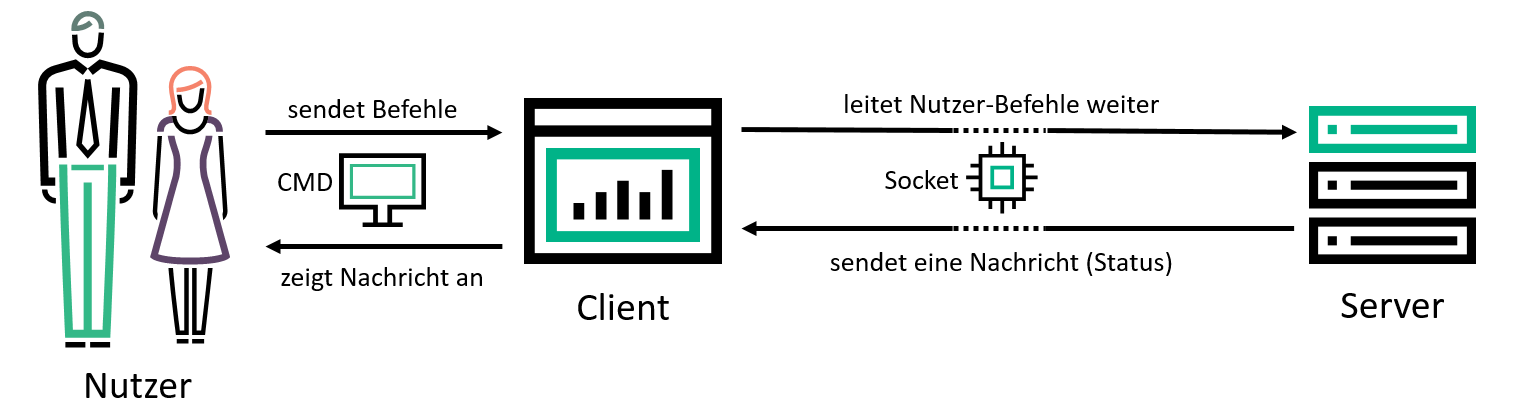
\includegraphics[scale=0.5]{Audioplayer_Konzept.png}
	\caption{Audioplayer - Konzept}
	\label{img:Konzept-Audioplayer}
\end{figure}

Das in Abbildung \ref{img:Konzept-Audioplayer} dargestellten Konzept spiegelt
eine übergreifende interaktive Sicht des Audioplayers wieder. Zudem sind in der
Abbildung alle für den Audioplayer benötigten Komponenten zu erkennen, wie:
\begin{itemize}
\item Nutzenden Personen
\item \ac{CMD}
\item Audioplayer-Client
\item Socket
\item Audioplayer-Server
\end{itemize}

Der Aufbau dieses Konzeptes wurde bewusst so gewählt, damit keine
Abhängigkeiten zwischen der Eingabe von Befehlen durch die nutzenden Personen
und den technischen Funktionen des Audioplayers zur Wiedergabe und Steuerung
der Audiodateien besteht. Daher sind der Client und der Server eigenständige
Programme die über einen Socket kommunizieren. Ein weiterer Vorteil dieses
Aufbau ist, dass theoretisch mehrere Nutzer den selben Audioplayer nutzen und
auch steuern können, was ganz neue Einsatzmöglichkeiten bietet. \\ 
Die nutzenden Personen stellen hier den späteren Bediener des Audioplayers da,
welche über eine Kommandozeilen-Programm (\ac{CMD} bzw. Shell) Befehle an den
Audioplayer-Client senden können. Die Befehle werden durch den Aufruf des
Client mit den entsprechenden Parametern übergeben. Der Client empfängt die
Befehle des Nutzers und und leitet diese als \ac{JSON} über einen vorher
erstellten Socket an den Server weiter. Der Server interpretiert den Befehl und
führt die gewünschte Aktion aus. Anschließend sendet der Server eine
Statusmeldung (Nachricht) an den Client zurück, welcher diese dem Nutzer über
das Kommandozeilen-Programm ausgibt. Danach danach beendet sich der Client
wieder - der Server läuft durchgängig weiter, bis dieser explizit durch einen
\enquote{Beenden} Befehl heruntergefahren wird. \\ 
Diese Beschreibung des
Konzeptes stellt nur eine grobe Übersicht der Funktionsweise dar, weshalb in
den nächsten Kapitalpunkten nochmals genauer auf den Client sowie den Server
und dem Socket eingegangen wird. Zusätzlich wird die Nutzung von
Konfigurationsdateien wie auch der Aufbau bzw. die Ordnerstruktur des
Audioplayers erläutert.

\subsection{Nutzung einer Konfigurationsdatei}
Unter einer Konfigurationsdatei versteht man in diesem Zusammenhang eine
Textdatei welche sich auf einem Computer befindet, in der bestimmte
Einstellungen für Computerprogramme gespeichert werden. Für die Speicherung
einer Konfigurationsdatei werden viele unterschiedliche Formate wie z.B.
\ac{INI}, \ac{YAML}, \ac{XML} oder \ac{JSON} verwendet
\autocite{hard_coding_and_soft_coding_2019} \autocite{lott_2019}. \\ 
Für den erstellten Audioplayer wurde eine Konfigurationsdatei in dem Format
\ac{JSON} verwendet um wichtige Einstellungen verändern zu können, ohne direkt
in den Programmcode eingreifen zu müssen. Aus diesem Grund befinden sich die
folgenden dargestellten Einstellungspunkte in unterhalb dargestellten \ac{JSON}
Datei. 
Json
\begin{lstlisting}[language=Json]
{
"Socket_Path" : "/tmp/mp.sock",
"Log_Dir": "logs/",
"Server_Log": "server.log",
"Server_Connection_Attempts": 10,
"Client_Log": "client.log",
"Default_Command": "default",
"Default_Depth": 2,
"Default_Input": "",
"Default_Loop": true,
"Default_Shuffle": false,
"Default_Volume": 50,
"Debug_Infos": true
}
\end{lstlisting}

Wie in dem Ausschnitt klar zu erkennen ist, werden einige Standardwerte für den
Audioplayer in der Konfigurationsdatei gespeichert, wie unter anderem z.B. den
Loop und Shuffle Status oder die Standardlautstärke wie auch die Tiefe für das
durchsuchen von übergebenen Ordnern. Zusätzlich werden dort auch noch die
Dateien bzw. Ordner angegeben in denen beispielsweise der Socket erstellt
werden soll oder die Log Dateien gespeichert werden sollen. Besonders zu
erwähnen ist, dass man über das Feld \verb|Debug_Infos| steuern kann, ob bei
der Ausführung des Audioplayers Debug-Informationen mit ausgegeben werden
sollen oder nicht. Dies ist gerade bei der weiteren Entwicklung des
Audioplayers von hoher Relevanz.

\subsection{Aufbau des Audioplayers}
Go besitzt einige Kodierrichtlinien, die dazu führen dass der geschriebene
Programmcode möglichst kurz, einfach und strukturiert ist. Um genau das zu
erreichen besitzt Go die Kodierrichtlinie zur Verwendung von sogenannten
\textit{packages}, welche zusammengehörigen Programmcode in eine extra Datei
bzw. ein \textit{Package} auslagert. In Go ist jeder Programmcode einem Package
zugeordnet. So ist z.B. das Hauptprogramm, also das Programm welches beim
starten eines Go-Programmes aufgerufen wird, immer im \enquote{main}-Package
ist. Sobald es einige zusammengehörige Funktionen, sei es Sinngemäß oder für
einen gewissen Zweck, in ein Package ausgelagert werden können, soll man dies
machen. Für jedes erstellte Package wird ein eigener Ordner in dem Verzeichnis
angelegt, wo dann alle zu dem Package zugehörige Dateien gespeichert werden.
Dabei kann ein Package aus mehreren Dateien bestehen die mehrere Funktionen
exportieren oder aus nur einer Datei die nur eine Funktion exportiert.
Zusätzlich sollte die Namenskonvention für Packages möglichst kurz aber
gleichzeitig noch verständlich sein \autocite{crawshaw_2019}. \\
Der Aufbau des Audioplayers wurde auf Basis dieser Kodierrichtlinie erstellt,
sodass sich die folgende Ordnerstruktur entwickelt:

\dirtree{%
.1 /. 
.2 logger. 
.3 logger.go. 
.2 portaudiofunctions. 
.3 portaudiofunctions.go.
.2 screener. 
.3 screener.go. 
.2 sender. 
.3 sender.go.
.2 serverfunctions. 
.3 audiofunctions.
.4 audiofunctions.go.
.3 connectionfunctions.
.4 connectionfunctions.go.
.3 volumefunctions.
.4 volumefunctions.go.
.2 structs.
.3 structs.go.
.2 util.
.3 util.go.
.2 config.json.
.2 MusicPlayerClient.go.
.2 MusicPlayerServer.go.
}

Die Hauptprogramme, also der Server und der Client, sowie die erstellte
Konfigurationsdatei liegen dem \textit{Root-Verzeichnis} des Audioplayers. Wie
zu erkennen, stellen die restlichen Ordner mit den beinhaltenden Dateien
jeweils einzelne Packages dar, die von den Hauptprogrammen wie aber auch von
anderen Packages genutzt werden können. \\
Im folgenden wird kurz zu jedem Package eine kleine Beschreibung folgenden.
\begin{enumerate}
\item \textbf{logger-Package} \\
Dieses Package wird von fast allen Funkionen des Audioplayers genutzt um die
Logdateien zu erstellen. Zudem bietet es auch Funktionen zu initialisieren des
Loggers.

\item \textbf{portaudiofunctions-Package} \\
In diesem Package sind alle Funktionen die für die Verwendung der
Portaudio-Bibliothek notwendig sind vorhanden. 


\item \textbf{screener-Package} \\
Das screener-Package besitzt Funktionen welche den Nutzer einen Start- und
Endbildschirm bei der Verwendung des Audioplayers anzeigt.


\item \textbf{sender-Package} \\
Das sender-Package beinhaltet die Funktionen zum Senden und Empfangen von
JSON-Nachrichten für den Client über den Socket.


\item \textbf{audiofunctions-Package} \\
Innerhalb des audiofunctions-Package sind alle implementierten Funktionen von
dem Audioplayer rund um das Abspielen von Audiodateien vorhanden.

\item \textbf{connectionfunctions-Package} \\
Hier sind die Funktionen für das Erstellen des Sockets sowie das Senden,
Empfangen und Schließen des Sockets vorhanden. Dies wird für den Kommunikation
zwischen Client und Server benötigt.

\item \textbf{volumefunctions-Package} \\
Durch dieses Package kann die Lautstärke für die Wiedergabe von Audiodateien
mit verändert werden.

\item \textbf{structs-Package} \\
Um einheitliche Strukturen von Daten zu haben, die sowohl der Client wie auch
der Server nutzen können, wurde das structs-Package erstellt welche
Datenstrukturen als \textit{struct} beinhaltet.

\item \textbf{util-Package} \\
In dem Package befinden sich sämtliche Funktionen die einen hilfreichen und
nützlichen Part haben und meist von mehreren Packages genutzt werden. Zum
Beispiel eine Funktion die kontrolliert ob eine gewissen Zeichenfolge sich in
einem String-Array befindet.
\end{enumerate}



\subsection{Konzept des Clients}
Wie bereits schon zuvor erklärt, hat der Client die Aufgabe die Befehle für den
Audioplayer vom Nutzer entgegenzunehmen und diese an der Server über einen
Socket weiterzuleiten.

\begin{figure}[H]
    \begin{struktogramm}(160,75)[Main-Funktion] 
        \assign{\hfill Konfigurationsdatei auslesen\hfill} 
        \assign{\hfill Aufsetzen des Loggers\hfill}
        \ifthenelse[12]{2}{1} {Überprüfen ob Server bereits läuft}{Ja}{Nein} 
        	\change
            \assign[5]{\hfill Starten des Servers\hfill}
        \ifend
        \ifthenelse[15]{2}{1} {Überprüfen ob Übergabeparameter übergeben wurden}{Ja}{Nein} 
        	\assign{\hfill Parsen der Informationen in ein JSON Format\hfill}
            \assign{\hfill Senden des JSONs and den Server\hfill}
            \while[5]{Bis Nachricht vom Server kommt}
            	\assign{\hfill Warten...\hfill}
            \whileend
            \assign{\hfill Anzeigen der Nachricht vom Server\hfill}
            \change
        \ifend
        \assign[5]{\hfill Beenden des Clients\hfill}
    \end{struktogramm} 
\caption{Client Programm - Ablauf} 
\label{lst:client_ablauf} 
\end{figure}

In der Abbildung \ref{lst:client_ablauf} wird der Programmablauf des Clients in
einem Struktogramm dargestellt und nun kurz erläutert. Als ersten Schritt ließt
der Client die zuvor erläuterte Konfigurationsdatei ein und initialisiert
anschließend den Logger, um alle folgenden ausgeführten Aktionen im Client in
einer Logdatei zu protokollieren. Anschließend wird überprüft ob ein Prozess
des Serverprogramms bereits existiert und läuft. Falls dies nicht der Fall ist,
startet der Client das Serverprogramm und wartet, bis der Server hochgefahren
ist und eine Verbindung über den Socket zum Server besteht. Sobald eine
Verbindung besteht, wird überprüft ob Übergabeparameter bei dem Aufruf des
Client mit übergeben wurden sind. Wurden keine Parameter übergeben, wird eine
Statusmeldung angezeigt und das Clientprogramm beendet sich. Falls jedoch
Parameter übergeben wurden sind, werden diese Informationen (Befehle) in ein
\ac{JSON} Format geparst und anschließend über den Socket an den Server
gesendet. Der Client wartet nun solang, bis er eine Antwort vom Server bekommt,
dass der Befehl ausgeführt wurden ist welches durch eine entsprechende
Statusmeldung an den Client realisiert wurde. Die Statusmeldung wird dem Nutzer
angezeigt worauf sich kurze Zeit später der Client automatisch beendet.

\subsection{Konzept des Servers}

Der Server stellt das \enquote{Herz} des Audioplayers dar. Nach einmaligem
starten des Servers, läuft dieser permanent als Prozess im Hintergrund und
setzt die Funktionen des Audioplayers um.

\begin{figure}[H]
    \begin{struktogramm}(160,80)[Main-Funktion] 
        \assign{\hfill Konfigurationsdatei auslesen\hfill} 
        \assign{\hfill Aufsetzen des Loggers\hfill}
        \assign{\hfill Aufsetzen des Sockets\hfill}
        \while[5]{Endlosschleife}
        	\assign{\hfill Abhören des Sockets auf Nachrichten\hfill}
        	\ifthenelse[12]{5}{1} {Nachricht erhalten}{Ja}{Nein}
        	    \assign[5]{\hfill Entpacken der Nachricht\hfill}
        	    \ifthenelse[12]{6}{5} {Befehl == \enquote{Beenden}}{Ja}{Nein}
        	    	\assign[5]{\hfill Nachricht an Client senden\hfill}
        	    	\assign[5]{\hfill Beenden der Wiedergabe\hfill}
        	    	\assign[5]{\hfill Schließen des Sockets\hfill}
        	    	\assign[5]{\hfill Beenden des Servers\hfill}
        	    	\change
        	    	\assign[10]{\hfill Ausführen des Befehls\hfill}
        	    	\assign[10]{\hfill Nachricht an Client senden\hfill}
        	    \ifend
        		\change
        	\ifend
        \whileend
    \end{struktogramm} 
\caption{Server Programm - Ablauf} 
\label{lst:server_ablauf} 
\end{figure}

In der Abbildung \ref{lst:server_ablauf} wird, wie bereits beim Client zuvor
auch, der grobe Programmablauf des Server dargestellt und im folgenden noch
kurz erläutert. Als ersten Schritt liest der Server, genau wie der Client, die
Einstellungen aus der Konfigurationsdatei aus und setzt anschließend den Logger
zum protokollieren der entstehenden Ereignisse auf. Darauf folgend setzt der
Server den Socket für die Kommunikation mit dem Client auf, wozu er den in der
Konfigurationsdatei festgelegten Pfad zur Erstellung des
Kommunikationsendpunktes nutzt. Sobald der Socket aufgesetzt ist und läuft,
beginnt der Server in eine Endlosschleife zu fallen, die folgende Funktionen
beinhaltet: Der Server hört die ganzen Zeit den Socket ab und wartet darauf das
Nachrichten eintreffen. Falls eine Nachricht eingetroffen ist, wird die
eingetroffene Nachricht welche in einem \ac{JSON} Format von Client kommt
geparst um die darin liegenden Informationen auslesen zu können. Im Falle
dessen, dass als Befehl das beenden des Server gefordert ist, wird zuerst eine
Bestätigungsnachricht an den Client zurückgesendet und anschließend die falls
vorhandene aktuelle Wiedergabe einer Audiodatei gestoppt und der Socket sowie
das Serverprogramm beendet. Andernfalls, wird der gewünschte Befehl vom Server
ausgeführt und nach erfolgreicher Ausführung eine Statusmeldung an den Client
zurück gesendet.
	

\section{Kommunikation über Sockets}
Eines der größten Schwierigkeiten in diesem Projekt war es ein Programm zu
entwickeln, was einerseits eine Audiodatei abspielt und gleichzeitig noch
Befehle entgegennehmen kann jedoch dazu aber nicht das System blockiert, sodass
nichts anderes mehr getätigt werden kann. Um dies zu ermöglichen wurde sich für
das bereits beschriebene Konzept aus Server und Client entschieden, die über
einen Socket kommunizieren. \\
Ein \textit{Socket} ist ein Kommunikationsendpunkt der vom Betriebssystem als
Objekt bereitgestellt wird. Programme verwenden meistens Sockets um mit anderen
Programmen Daten auszutauschen und miteinander zu kommunizieren. Dies ist
unabhängig davon, ob beide Programme sich auf dem selbem Computer oder einem
anderen, über das Netzwerk erreichbaren Computer befinden. Sockets
kommunizieren in der Regel bidirektional, was bedeutet, dass über den Socket
sowohl Daten gesendet wie auch empfangen werden können. Technisch ist der
Socket ein Speicherbereich in dem Konfigurationsparameter einer Verbindung wie
auch ankommende und abgehende Daten zwischengespeichert werden. Aufgrund
dessen, dass ein Socket vom Betriebssystem bereit gestellt wird, hat man keinen
direkt zugriff auf den Socket sondern kann nur über Funktionen der
Programmiersprache auf den Socket zugreifen.
Ein Socket wird immer von einem Programm bei Bedarf erstellt und ist somit
diesem Prozess fest zugeordnet \autocite{pollakowski_2012}. \\
Dies erlaubt es, dass der Server im Hintergrund Befehle entgegennehmen und
Audiodateien abspielen kann und dabei nicht das System "blockiert". Der Client
der über den Socket mit dem Server kommuniziert wird immer nur für die
Übertragung eines Befehl übertragen und hat damit nur die Aufgabe den Server
mit neuen Befehlen zu füllen.

\section{Funktionen des Audioplayers}
Nachdem nun die Konzepte zur Umsetzung des Audioplayers beschrieben wurden,
wird nun auf die jeweiligen Funktionen des Audioplayers eingegangen. Dabei wird
zu jeder Funktion eine kurze Beschreibung sowie die Syntax für den Aufruf
erläutert.

\definecolor{Gray}{gray}{0.9}
\begin{longtable}{l|l} 
\rowcolor{Gray}
Funktion & Beschreibung \\ \hline

Audio abspielen & \begin{minipage}[t]{.558\textwidth} Zur Wiedergabe einer Audiodatei kann entweder ein einzelner Song oder eine gesamter Ordner als Pfad angegeben werden. Im Falle eines Ordners, wird eine Playlist mit den darin liegenden Audiodateien erstellt und wiedergegeben. \begin{lstlisting}
./MusicPlayerClient play [File/Folder Path]
\end{lstlisting} \end{minipage} \\\hline

Audio pausieren & \begin{minipage}[t]{.558\textwidth} Der Audioplayer bietet die Möglichkeit einen aktuell laufenden Song zu pausieren. Technisch gesehen wir dabei der Stream(Das Decoden der Datei) pausiert sodass keine Ausgabe mehr erfolgt. \begin{lstlisting}
./MusicPlayerClient pause
\end{lstlisting} \end{minipage} \\ \hline

Audio fortfahren & \begin{minipage}[t]{.558\textwidth} Nachdem der Befehl zum pausieren eines laufenden Song ausgeführt wurde, kann der Song auch ab der pausierten Stelle wieder fortgesetzt werden. Der Befehl funktioniert nur wenn ein Lied pausiert ist. \begin{lstlisting}
./MusicPlayerClient resume
\end{lstlisting} \end{minipage} \\ \hline

Audio stoppen & \begin{minipage}[t]{.558\textwidth} Das stoppen einer Wiedergabe bewirkt, dass das aktuell laufende Lied angehalten wird aber sich nicht der Zeitpunkt gespeichert wird. Bei erneutem Starten beginnt der Song wieder von vorne. \begin{lstlisting}
./MusicPlayerClient stop
\end{lstlisting} \end{minipage} \\ \hline

Audio-Weiter & \begin{minipage}[t]{.558\textwidth} Falls eine Ordner übergeben wurden ist oder manuell eine Playlist erstellt wurde, kann durch den folgenden Befehl das akutelle laufende Audio gestoppt werden und das nächste Lied in der Playlist wird automatisch gestartet. \begin{lstlisting}
./MusicPlayerClient next
\end{lstlisting} \end{minipage} \\ \hline

Audio-Zurück & \begin{minipage}[t]{.558\textwidth} Äquivalent zur Funktion Audio-Weiter, wird bei dieser Funktion das aktuell lafende Audio gestoppt und das sich vorherige in der Playlist befindliche Audio wiedergegeben.  \begin{lstlisting}
./MusicPlayerClient back/previous
\end{lstlisting} \end{minipage} \\ \hline

Audio zur Playlist hinzufügen &  \begin{minipage}[t]{.558\textwidth} Falls bereits eine Playlist besteht oder eine neue dadurch erstellt werden soll, kann über diesen Befehl ein Audio oder ein Ordner mit den darin liegenden Audios der Playlist angefügt werden. \begin{lstlisting}
./MusicPlayerClient add/addToQueue [File/Folder path]
\end{lstlisting} \end{minipage} \\ \hline

Audio von Playlist löschen & \begin{minipage}[t]{.558\textwidth} Einzelne Audiodateien in einer Playlist können auch durch den folgenden Befehl wieder entfernt werden. Dazu muss die Nummer in der Playlist angegeben werden die bei der anzeige von Informationen mit ausgegeben wird. \begin{lstlisting}
./MusicPlayerClient remove/delete/removeAt/deleteAt [Queue number]
\end{lstlisting} \end{minipage} \\ \hline

Lautstärke festlegen & \begin{minipage}[t]{.558\textwidth} Die Lautstärke der Ausgabe der Audiodateien kann zwischen 0 und 100 eigentständig selbst bestimmt werden. Dabei mir technisch gesehen die Lautstärke des Audioausgangs des Raspberry Pi verändert. \begin{lstlisting}
./MusicPlayerClient setVolume [0-100]
\end{lstlisting} \end{minipage} \\ \hline

Lautstärke erhöhen & \begin{minipage}[t]{.558\textwidth} Um die Lautstärke nicht auf einen festen Wert zu setzen, kann auch einfach von dem akutellen Wert der Lautstärke um einen gewissen Grad erhöht werden. Bei jedem Aufruf dieser Funktion wird die Lautstärke um 10 Schritte erhöht. Maximal ist der Wert 100 möglich. \begin{lstlisting}
./MusicPlayerClient louder/setVolumeUp
\end{lstlisting} \end{minipage} \\ \hline

Lautstärke verringern & \begin{minipage}[t]{.558\textwidth} Um die Lautstärke nicht auf einen festen Wert zu setzen, kann auch einfach von dem akutellen Wert der Lautstärke um einen gewissen Grad verringert werden. Bei jedem Aufruf dieser Funktion wird die Lautstärke um 10 Schritte verringert. Minimal ist der Wert 0 möglich. \begin{lstlisting}
./MusicPlayerClient quieter/setVolumeDown
\end{lstlisting} \end{minipage} \\ \hline

Shuffle-Funktion & \begin{minipage}[t]{.558\textwidth} Die Shuffle-Funktion hat die Aufgabe die Audio in einer Playlist zufällig wiederzugeben. Dazu wird die Playlist per Zufall einmal neu durchgemischt, sodass eine Zufallswiedergabe stattfindet. Ein Aufruf bewirkt ein eimaliges durchmischen der Playlist. \begin{lstlisting}
./MusicPlayerClient shuffle/setShuffle
\end{lstlisting} \end{minipage} \\ \hline

Loop-Funktion de/-aktivieren & \begin{minipage}[t]{.558\textwidth} Durch das aktivieren/deaktivieren der Loop-Funktion wird eine Playlist nach dem durchlauf wieder von vorne beginnen, also eine Endloswiedergabe. Dies ist auch Möglich wenn nur ein einzelner Song wiedergegeben wird. \begin{lstlisting}
./MusicPlayerClient loop/setLoop [on,true/off,false]
\end{lstlisting} \end{minipage} \\ \hline

aktuellen Song neu starten & \begin{minipage}[t]{.558\textwidth} Durch diese Funktion wird die aktuell laufende Audio gestoppt und die gleiche Audio wieder von Anfang an wiedergegeben. \begin{lstlisting}
./MusicPlayerClient repeat
\end{lstlisting} \end{minipage} \\ \hline

Informationen ausgeben & \begin{minipage}[t]{.558\textwidth} Hiermit werden dem Nutzer einige Informationen zum Audioplayer wie z.B. die aktuell laufende Audio sowie den Inhalt der Playlist in einer Tabellenform. Dabei werden die Informationen aus den ID3 Tags der Audiodateien geholt. Zusätzlich werden die aktuellen Lautstärke Einstellungen ausgegeben \begin{lstlisting}
./MusicPlayerClient info
\end{lstlisting} \end{minipage} \\
\caption{Übersicht - Funktionen des Audioplayers} % needs to go inside longtable environment
\label{tab:funktionendesaudioplayer_longtable}
\end{longtable}

